\section{De nouveaux modèles de sociétés}

\paragraph{} Nos sociétés ont toujours été avides de \emph{contrôle}, et cela indépendamment du régime politique en 
place. 

\paragraph{} \guillemotleft La bourgeoisie a subordonné l'Orient à l'Occident. \guillemotright selon Marx et Engels,
mais \guillemotleft Le prolétariat utilisera sa domination politique pour arracher peu à peu tout le capital à la
bourgeoisie, pour centraliser tous les instruments de production entre les mains de l'Etat, c'est-à-dire du prolétariat
organisé en classe dominante.\guillemotright \cite{Marx1} Il apparaît ici clairement que leur vision
n'est qu'un énième renversement de la bascule des pouvoirs, sans déplacement du rapport de force. Pire que cela, la mise
en place d'un "État prolétaire totalitaire" vise à faire disparaître l'individu (le \emph{Soi}) au profit d'un \emph{Nous}
qui se ferme aux différences : homogénéisation de la classe dominante, refus - voire peur - de l'autre, ce schéma semble
se représenter de manière cyclique à travers les âges.

\paragraph{} L'analogie du modèle carcéral de Foucault souligne elle aussi ces tendances extrêmes.
En effet, les exécutions et supplices publiques étaient un moyen de corriger le tort causé au souverain par le crime ou
délit ; ce dernier exprimait alors une possession pleine et entière de l'individu, et par extension des spectateurs. 
Le contrôle exercé était alors physique pour l'un et psychologique pour les autres, qui craignaient alors de se
retrouver un jour à sa place. Vinrent ensuite les travaux de force, le bagne, dont l'objectif n'était plus d'infliger
une souffrance directe mais d'affirmer une emprise plus entière sur les capacités physiques et mentales des condamnés.
Finalement, on cessera d'avoir recours au supplice pour privilégier l'enfermement. Il n'est pas alors question d'une
pudeur excessive à l'idée de punir, mais plutôt de resituer l'objectif réel de la punition.
\guillemotleft L'âme succède au corps comme objet de l'expiation des crimes. \guillemotright \cite{Foucault0}

\paragraph{À développer} Des supplices féodaux à l'enfermement à perpétuité, nos sociétés ont fait évoluer de manière perverse les
mécanismes de contrôle. Le développement du Panoptisme, d'abord comme architecture par les frères Bentham puis 
comme idéologie chez Foucault, fait croître le sentiment d'impunité de celui qui châtie. Se pensant inatteignable, il 
adaptera en conséquence son comportement vis-à-vis des autres, qui developperont à leur tour un sentiment constant
d'observation.

\begin{figure}[h]
    \centering
    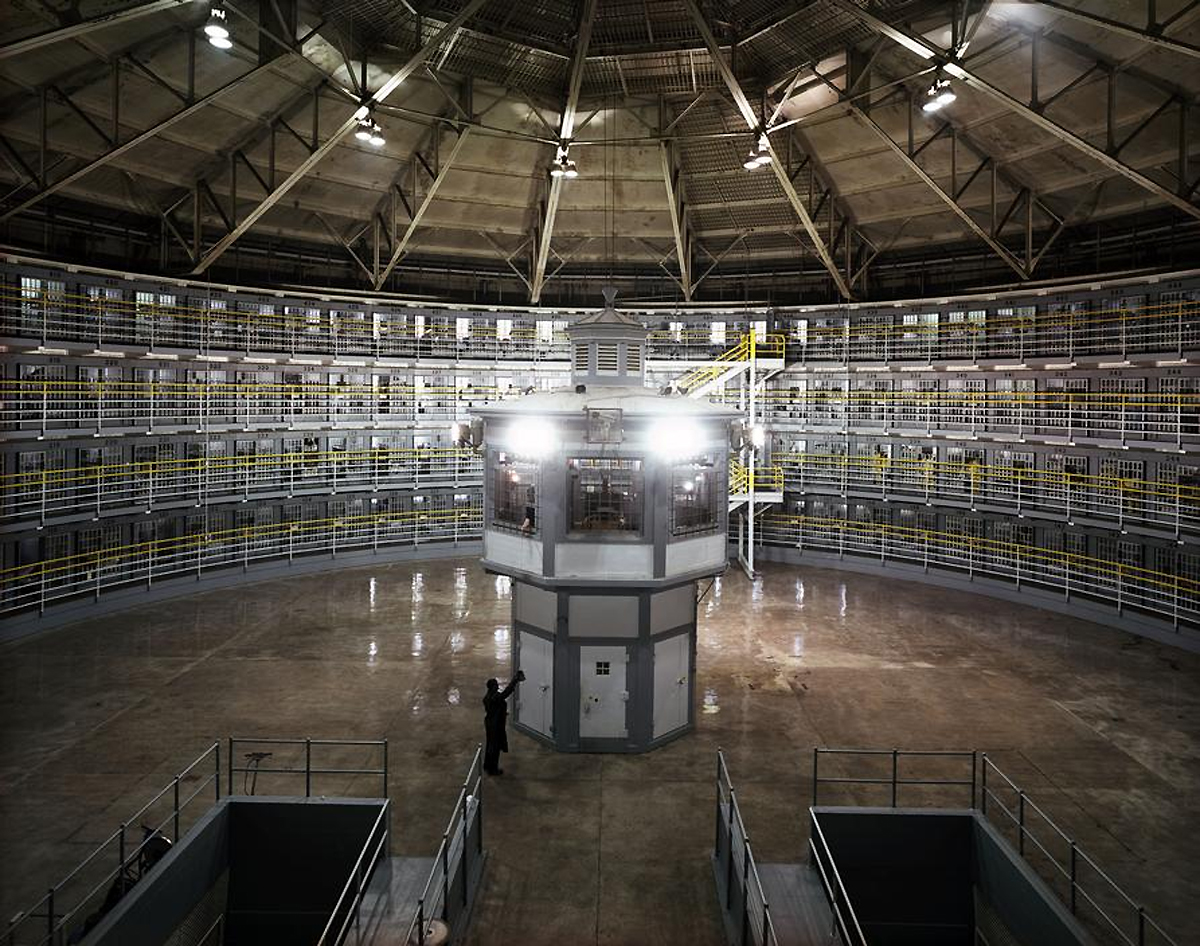
\includegraphics[scale=0.2]{images/panoptique.jpg}
    \caption{\label{Panoptique} Presidio Modelo, Cuba : Prison construite sur le modèle panoptique}
\end{figure}

\paragraph{} Mais de quoi sont faites les sociétés sinon d'Hommes ? De là, ce sont bien les aspirations de ceux qui les 
composent qu'elles reflètent à l'identique, et c'est justement cette volonté de contrôle que la technologie viendra par
la suite outiller.

\section*{Brouillon}

\paragraph{Références} \cite{Marx0} \cite{Marx1} \cite{Nietzsche0}

\paragraph{Ère pré-internet} Analyse des dernières décénnies du XX\up{ème} siècle :
comment les sociétés ont évoluées avec l'arrivée des nouvelles technologies : du
pré-internet à l'ère des réseaux ; jusqu'à aujourd'hui. Quels étaient les objectifs
premiers des ces technos. (la raison de leur développement) ? Comment ont-elles réellement
été utilisées/ont été amenées à évoluer ? Est-ce réellement une mauvaise chose (n'y
a-t-il que du mal qui en soit ressorti) ? Est-il pertinent/nécessaire d'effectuer un bref
historique des technologies \emph{disruptives} (machine de Turing, architecture
Von Neumann, premiers réseaux, ...) ?

\paragraph{L'individu technique} Comment les modèles de sociétés nous ont-ils amené à
réfléchir l'individu en termes technologiques ?

\paragraph{Objectif} L'objectif ici est de démontrer que, suite au développement des technologies, c'est l'Homme
qui génère lui-même des données le concernant, par l'utilisation au quotidien des services (entre autres).
Cela doit être démontré par la mise en place d'un prototype récupérant des données de différents
services (ie facebook, twitter...)

\paragraph{Damasio : Très humain plutôt que transhumain}

\begin{quotation}
    L'homme réinvente sans cesse ce qu'il est par la technologie. Nous réinventons notre
    rapport au monde, notre rapport aux autres ; peut être et même surtout notre rapport à soi, 
    notre construction de soi, par la technologie. \cite{Damasio2}
\end{quotation}

Extension de soi - dispositifs tactils et bienveillants autour de nous, qui nous assistent,
nous prolongent, et font de nous de jeunes dieux agiles auxquels le fantôme digital du monde répondrait
; au doigt, et à l'oeil - évidemment.

On y gagne une maitrise, un pouvoir accru sur le monde. Mais n'y perd-on pas quelque chose ?
La "puissance" de Spinoza : celle de vivre, d'agir, d'habiter le monde, de persévérer dans mon être.

Le pouvoir = faire faire - déléguer l'action.
La puissance = la capacité de faire - de déployer l'action par soi-même.

Image de l'oignon technologique, que l'on ne sait plus ni éplucher ni cuisiner à notre
sauce sans risquer de pleurer.

La technologie vient outiller nos paresses. Faciliter nos vies, les fluidifier : on lui
délègue nos efforts, on lui sous-traite nos fatigues. Externalisation des capacités physiques :
voitures, métro, tapis roulant, ... Externalisation des capacités cognitives dans la machine :
mémoire = moteur de recherche, orientation = GPS, organisation = applications de
calendrier/planning - c'est aujourd'hui notre quotidien.

La technologie conjure nos peurs, principalement celles de la solitude et de l'abandon :
le réseau, le portable. Plus jamais SEUL.

La technologie est une eau qui s'infiltre dans tous les interstices, dans tous les blancs,
dans tous les doutes, dans tous les temps morts angoissés de nos vies pour les combler.
On lui demande de pouvoir contrôler notre environnement. Tout bouge sans que rien n'arrive. 

La technologie donne l'espoir de dépasser notre finitude. Le transhumanisme vise à
externaliser dans la technique ce que notre chaire et notre esprit ne sont supposément
pas capables de faire par eux-même.

La technologie ne nous pousse pas à *agir*, mais à *réagir* à des stimulis extérieurs :
notifications, mails, SMS, discussions instantanées, ...

Agir, c'est produire un événement qui libère un peu de vie là où les dispositifs de contrôle
l'étouffe en la gérant. C'est sentir qu'indépendamment de nos outils, nous sommes une puissance.


\section*{Prototype}

\paragraph{} Pour étayer notre propos, un prototype servira de fil rouge tout au
long de votre lecture. Nous nous intéresserons ici à la récupération de données personnelles,
focus de cette première partie. Pour cela, nous avons restreint notre champs d'action à quelques
services pertinents pouvant nous apporter un maximum d'informations :

\begin{itemize}
    \item Facebook : récupération des données publiques des profils utilisateurs ;
    \item Twitter : récupération du profil et des derniers messages de l'utilisateur, jugés
    représentatifs de son \emph{opinion} ;
    \item Instagram : récupération des photos de l'utilisateur ; 
    \item Google Maps API : récupération des coordonnées géographiques associées à une adresse
    (\url{https://maps.google.com/maps/api/geocode/json?address={ADDRESS}}) ;
    \item Google : récupération des suggestions de pages liées à la personne concernée par le
    premier moteur de recherche mondial (\url{https://encrypted.google.com/search?q={SEARCH_TERMS}}) ;
    \item LinkedIn : récupération du profil professionnel de l'utilisateur (\emph{nécessite une clé d'API ?}).
\end{itemize}

\paragraph{} Afin de permettre une aggrégation simple de l'ensemble de ces données, une 
API REST sert de façade pour d'éventuelles applications ou un usage à des fins de recherche
par un être humain. La récupération concertée des informations concernant une personne peut
être effectuée grâce à une requête \lstinline{GET} sur l'URL \url{https://{API_URL}/people/{NAME}}
- la réponse est au format JSON.

\paragraph{} En arrière plan, plusieurs composants entrent en jeu. Pour chacun des services
ci-dessus, un \emph{récupérateur} dédié a la charge de l'obtention et du formatage des données
exposées. Ces différentes informations sont ensuite retravaillées et aggrégées de manière 
à créer un "\emph{profil utilisateur}" le plus complet possible à partir des informations
disponibles publiquement sur internet.

\paragraph{} Pour cette première version de notre prototype, aucun \emph{état} ni aucune
donnée ne sont persistés. Les \emph{endpoints} de notre API sont les suivants :

\begin{itemize}
    \item \url{/people/{NAME}}
    \item \url{/services/facebook/{NAME}}
    \item \url{/services/twitter/{NAME}}
    \item \url{/services/instagram/{NAME}}
    \item \url{/services/google/{NAME}}
    \item \url{/services/linkedin/{NAME}}
\end{itemize}